\documentclass[main.tex]{subfiles}
\begin{document}
\chapter{Biologie du cancer}
\todo{lettrine}

\section{Le développement métastatique}

\section{Un scanner~: Comment ça marche ?}

\section{STAGE M1 : Un peu de biologie}
\subsection{Croissance tumorale}
Une tumeur est un ensemble de cellules de l'organisme se multipliant de manière dégénérée. Certains scientifiques s'accordent à dire que cela partirait d'une seule cellule (pour l'instant aucune preuve de cela n'a encore été apportée~: le sujet reste ouvert). Chaque cellule fille est alors à son tour dégénérée et se multiplie encore et encore. La tumeur grandit alors exponentiellement. En réalité, la croissance tumorale est limitée par les besoins de glucose et d'oxygène. En effet, à force de se multiplier les cellules sont en surpopulation. Les nutriments et l'oxygène viennent à manquer : c'est l'hypoxie. Les cellules du bord de la tumeur consomment tout et n'en laissent pas assez pour celles situées plus au centre. C'est dans ces cas là que l'on peut voir sur les scanners des tumeurs avec 2 nuances de gris~:
\begin{itemize}
\item Un gris foncé au centre, emplacement du tissu en partie nécrosé
\item Un gris plus clair sur le pourtour, lieu de la prolifération
\end{itemize}

\hrule
La tumeur en grandissant, va pousser vers l'extérieur le réseau sanguin qui l'alimente ! (La tumeur exerçant une pression sur celui-ci). \todo{valable que pour les méta, tumeur primit=infiltrante}
\hrule

\newpage
\begin{wrapfigure}[18]{R}{.5\textwidth}
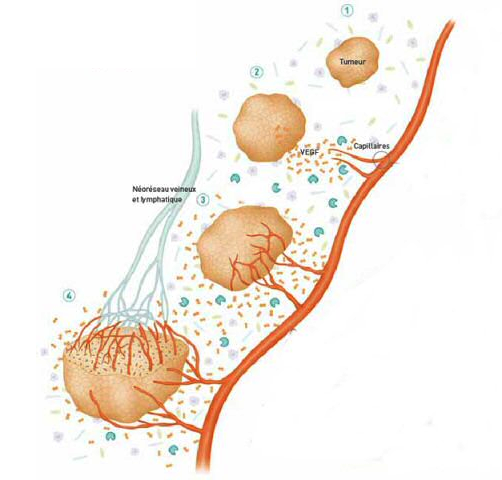
\includegraphics[width=.5\textwidth]{schema/angiogenese.jpg}
\captionof{figure}{\label{fig:schema_angio} Schéma descriptif de l'angiogénèse générant la néovascularisation \cite{web1}.}
\end{wrapfigure}
Les cellules en hypoxie vont alors entrer dans un état de quiescence et vont sécréter des facteurs de croissance, dont le VEGF (Vascular Endothelial Growth Factor). Ces protéïnes commandent la création de nouveaux vaisseaux sanguins, processus appellé \emph{angiogenèse}. Les facteurs de croissances sont destinés aux cellules endothéliales, cellules qui recouvrent la paroi intérieure des vaisseaux sanguins et directement impliquées dans l'angiogenèse. Ces cellules vont construirent des nouveaux vaisseaux sanguins par chimiotactisme~: les nouveaux vaisseaux sanguins sont orientés dans le sens où la concentration de facteur de croissance est la plus forte. Ainsi la tumeur se créée son propre réseau sanguin~: la \emph{néovascularisation}. La nourriture et l'oxygène redeviennent de nouveau abondants. 
Les cellules qui étaient en hypoxie \todo{cellule normale -> apoptose} vont alors se remettre à proliférer jusqu'à ce que de nouveau, il y ait surpopulation. Et ainsi de suite, le cycle continue. On peut visualiser ce cycle sur le schéma présenter Figure~\ref{fig:schema_angio}.\\


\begin{wrapfigure}[17]{l}{.5\textwidth} %%% L : Left flottant / l: left non flottant (pas de pagebreak)
\setlength{\unitlength}{.005\textwidth}
\vspace{-9mm}
\begin{picture}(100,93)
\tiny 
\put(0,2){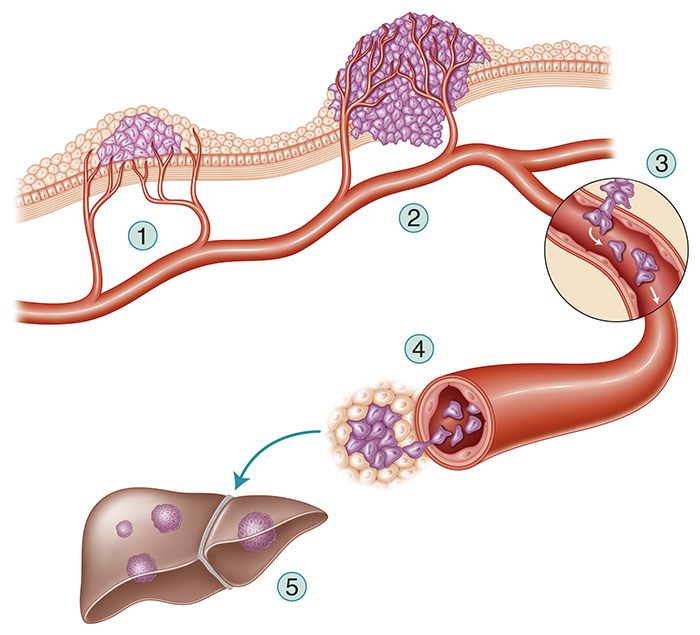
\includegraphics[width=.5\textwidth]{schema/cellules_tumorales_circulantes_copyright.jpg}}
\put(30,0){Copyright Eléonore Lamoglia/Institut Curie}
%%\put(0,0){\rect{0}{0}{100}{93}}
\end{picture}
\captionof{figure}{\label{fig:schema_dissemination_metastase} Dissémination des métastases.}
\end{wrapfigure}
Bien que la tumeur cherche continuement à se vasculariser toujours plus, paradoxalement, sa croissance va endommager le réseau sanguin qui l'irrigue. Une partie des cellules tumorales (cellules invasives) va alors pouvoir pénétrer dans les voies sanguines. La plupart de ces essaims seront éliminés par le système immunitaire. Une partie arrivera à s'installer dans un autre organe~: elle forment des tumeurs filles appelées~\emph{métastases}. De simple cellules ne pourraient pas nicher dans un autre organe que celui auquel elles appartenaient au départ. Les cellules tumorales le peuvent, car à force de division elles s'indifférencient. C'est-à-dire qu'elles s'approchent de ce qu'elles étaient au stade embreyonnaire~: des cellules souches qui en se différenciant formeront aussi bien des cellules de l'intestin que des cellules du foie. Ce type de cellules, bien que provenant de l'intestin, n'est donc pas reconnu comme étranger au foie et la métastase peut s'installer.

\subsection{Les traitements}
A l'heure actuelle aucun traitement ne permet de guérir le cancer. Cependant plusieurs techniques existent pour prolonger et/ou améliorer la vie des patients.
\paragraph{La chirurgie} ne peut-être réalisée que sur des cancers primaires, non métastasés et donc détectés tôt. C'est la première option considérée par le corps médical (bien que la chirurgie elle-même puisse être source de dissémination de métastase, \cf par exemple  \url{http://www.sciencedirect.com/science/article/pii/S0748798305000089}).

\paragraph{L'ablation par radiofréquence} permet, à l'aide d'une sonde électromagnétique à haute fréquence, de bruler une région définie par le médecin. On peut ainsi réaliser une ablation sans avoir à opérer le patient. Cette technique  
ne peut cependant être utilisée que pour de petite tumeur, ne dépassant pas une certaine taille (de l'ordre du centimètre \todo{A verif, ref?}) et n'étant pas à proximité d'organes sensibles. 

\paragraph{La radiothérapie} consiste à irradier une zone de l'organisme par une forte dose de rayons X. Ceci a pour effet de détruire les cellules qui se multiplient, et donc par voie de conséquence, les cellules cancéreuses. Cette méthode présente les mêmes limitations que la radiofréquence à savoir que son efficacité est limité à des petites tumeurs. La radiothérapie est souvent utilisé à titre paliatif sur des petites métastases (pulmonaires notamment).

\paragraph{Les thérapies ciblées} sont des médicamments administrés par voies intraveineuses. Ces thérapies sont ciblées, non pas dans le sens où elle ne vont s'orienter que vers les cellule cancéreuses (bien au contraire elles se répandent dans tous l'organisme), mais dans le sens où elles vont inhiber un type spécifique de voies moléculaires (ou de récepteurs). En exemple on pourra citer l'\emph{imatinib} (Glivec) qui se fixe sur les récepteurs cellulaires (récepteurs de tyrosine kinase, RTK) commandant l'activité intra cellulaire. En inhibant ces récepteurs, l'apoptose tends à se réactiver dans les cellules défectuesues. On peut également cité en exemple le bevacizumab (Avastin), qui inhibe l'angiogenèse. D'autres molécules ont plusieurs effets ciblés. Le sorafenib ou le sunitinib en font parties.\\
sorafenib (Nexavar) =  TKI (Raf-kinase, intervenant dans la cascade de kinases activées lors de la mitose) + VEGFR \\
sunitinib (Sutent) =  KIT inhib (CD117, the RTK that drives the majority of gastrointestinal stromal cell tumors ) + VEGFR \\


============= deb rapportstage M2 ==============\\

\subsubsection{La chimiothérapie}
La chimiothérapie est l'injection dans le sang d'une substance chimique modifiant la forme de l'ADN de l'ensemble des cellules de l'organisme. Ceci a pour effet que toute cellule voulant se diviser péri. Ceci permet de limiter donc la croissance de la tumeur. Cependant le traitement agit sur toutes les cellules, et donc sur les cellules saines également. Ce qui n'est pas sans laissé d'effets secondaires. L'organisme ne peut plus fabriquer de nouvelle cellules là où il y en a besoin, ce qui se traduit par la perte des cheveux, etc \ldots

\subsubsection{Les anti-angiogéniques}\label{trait antiangio}
Les anti-angiogénique sont des molécules inhibitrices de l'angiogenèse. Les antiangiogéniques peuvent être classés , selon leur mode d'action, en deux catégories :
\begin{enumerate}
\item Les protéïnes se placent sur les récepteurs spécifiques à la VEGF sur les cellules endothéliales, inhibant ainsi l'effet de la VEGF.
\item Ou bien elles se placent directement sur la VEGF, l'empêchant ainsi de se fixer aux cellules endothéliales.
\end{enumerate}
 En administrant des anti-angiogénique au patient, on prive alors l'organisme de la création de nouveaux vaisseaux sanguins. La tumeur ne peut alors plus s'alimenter. Ceci n'est pas non plus sans effet secondaires : difficultés de cicatrisation par exemple. Les anti-angiogéniques ont pour effet également de renforcer le réseau sanguin existant. Ceci limite donc la dissémination des métastases par voie sanguine, car celles-ci ont beaucoup plus de mal à entrer dans le réseau.

\subsection{Chimiothérapie et anti-angiogéniques}
Il s'avère qu'une chimiothérapie seule est assez inefficace. En effet, en grandissant la tumeur détériore le réseau sanguin qui l'alimente. Le traitement arrivant par voie sanguine n'a donc aucune chance d'atteindre le centre de la tumeur. En cumulant chimiothérapie et anti-angiogéniques, le réseau sanguin est consolidé et nettement moins endommagé par la tumeur ce qui permet à la chimiothérapie d'atteindre le coeur de la tumeur et ainsi agir de manière efficace.\\
=============   FIN RAPPORT STAGE M1  ===========\\


\section{Fonctionnement du scanner}
Le scanner est un examen médicale qui permet d'acquérir des images d'une partie de l'organisme par le biais d'une irradiation aux Rayons~X. Oui, oui, une irradiation ! Cependant l'irradiation est faible et de plus en plus d'études mettent en avant des méthodes pour la réduire  \url{http://www.ncbi.nlm.nih.gov/pmc/articles/PMC2743386/} ). Le bénéfice est donc très important devant les risques marginaux. C'est certainement l'une des raisons pour laquelle le scanner (tout comme la radio, ou l'IRM) est aujourd'hui très utilisé pour diagnostiquer une maladie, ou ne serait-ce même que pour contrôler la santé d'un patient.


\begin{wrapfigure}[18]{r}{.3\textwidth} %%% L : Left flottant / l: left non flottant (pas de pagebreak)
\vspace{-5mm}
\setlength{\unitlength}{.0032\textwidth}
\begin{picture}(100,121)
\scriptsize
%\footnotesize
\put(0,0){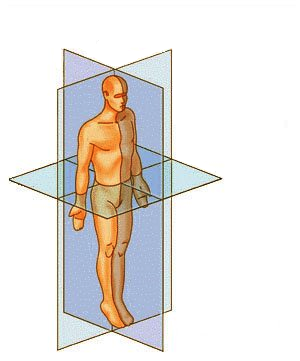
\includegraphics[width=.32\textwidth]{schema/Coupe_anatomie.jpg}}
\put(37,113){\vector(-1,-1){10}}
\put(69,100){\vector(-1,-1){10}}
\put(75,46){\vector(-1,1){10}}
\put(0,115){Plan sagital (ou frontal)}
\put(71,102){Plan}
\put(71,95){coronal}
\put(72,39){Plan}
\put(66,32){axial (ou}
\put(64,25){transverse)}
%%\put(100,0){\line(0,1){121}}
\end{picture}
\captionof{figure}{\label{fig:schema_coupe} Plans de coupe du corps humain.}
\end{wrapfigure}
Un scanner procède par acquisition d'images en couches. En ce qui concerne le scanner du thorax, le patient est \og découpé \fg{} de part en part 
\url{http://www.impactscan.org/download/msctdose.pdf}
\lipsum[1]

Chaque constituant de l'organisme à sa propre

\begin{figure}[h]
\setlength{\unitlength}{0.01\textwidth}
\begin{picture}(100,100)
\put(0,0){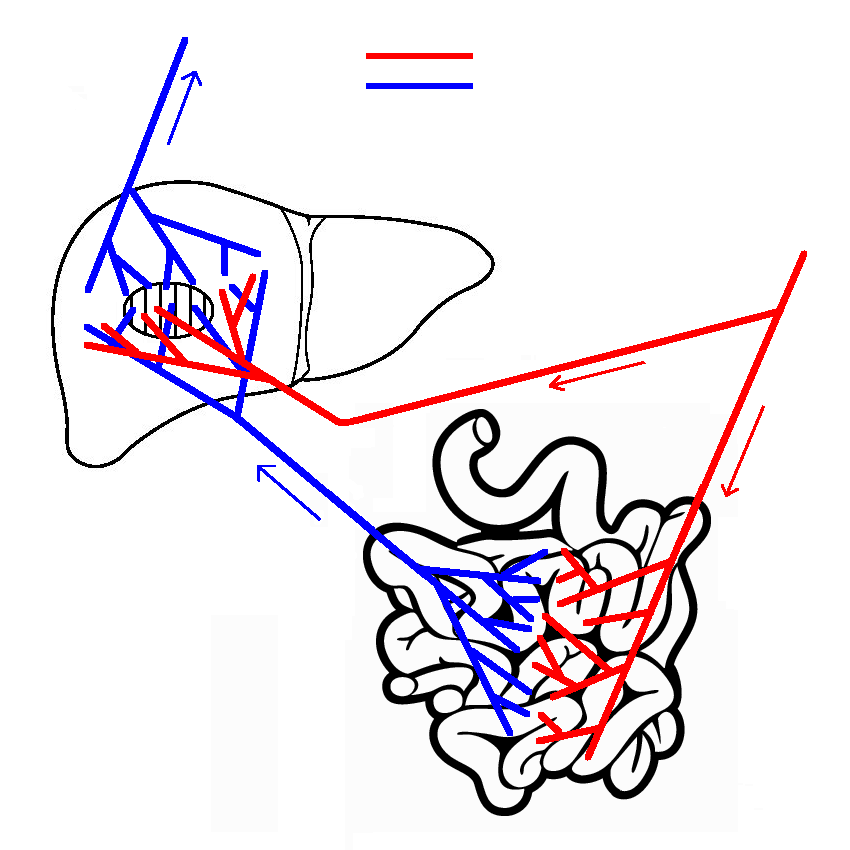
\includegraphics[width=100\unitlength]{schema/schema_irrigation_foie.png}}

%%% Cadre bordure
%\put(0,0){\line(0,1){100}}\put(0,0){\line(1,0){100}}
%\put(100,0){\line(0,1){100}}\put(0,100){\line(1,0){100}}

\put(57,92.5){Sang artériel, riche en oxygène}
\put(57,89){Sang veineux, pauvre en oxygène}

\put(40,75){Foie}
\put(82,18){Intestin grêle}
\put(82,15){et autres}
\put(83,12){organes du}
\put(82,9){tube digestif }

\linethickness{0.4\unitlength}
\put(18,65){\line(-10,-30){10}}
\put(1,32){Métastase}
\put(1,29){hépatique}

\put(57,56){ \begin{turn}{15} Artère hépatique \end{turn} }
\put(11,78){ \begin{turn}{70} Veine hépatique \end{turn} }
\put(31,49){ \begin{turn}{-40} Veine porte \end{turn} }
\put(77.5,48){ \begin{turn}{66} Artère \end{turn} }
\put(79,44){ \begin{turn}{66} mésentérique \end{turn} }
\end{picture}

\vspace{-10mm}
\caption{\label{fig:schema_irrig_foie} Schéma de l'irrigation du foie.}
\end{figure}
\end{document}